\chapter{Oide effect}\label{s:Oideeffect}
This part of the document addresses the radiation phenomenon in quadrupoles called Oide effect\cite{Oide}, which sets a limit on the beam size demagnification, specially important in linear colliders because of the strong focusing required in the Final Doublet before the Interation Point (IP).\par
First, a brief introduction to the beam size limit (Oide limit) is given, where calculations have been derived to include this radiation phenomenon in the lattice design and optimization software. The Oide effect is evaluated for the CLIC 3 TeV and CLIC 500 GeV parameters, leading to change the length of the first quadrupole before the IP, called QD0. It ends with a proposal to mitigate the impact of the Oide effect by adding correctors before and after the QD0, reducing the beam size.\par
\section{Beam size limit}\label{Oideeffect}
The Oide effect is caused by the interaction of charged particles with the magnetic field from quadrupoles. Radiation in a focusing magnet, schematically represented as QD0 in Fig. (\ref{f:Oideeffect}), changes the energy of the particle and modifies the focusing effect. This results in a limit on the minimum beam size specially relevant in the vertical plane.\par%For the horizontal direction, is mainly affected by radiation caused by the interaction of charged particles with the magnetic field from dipoles. %This report will be limited to sector dipoles or ``sbends''.\par
\begin{figure}[!hbt]
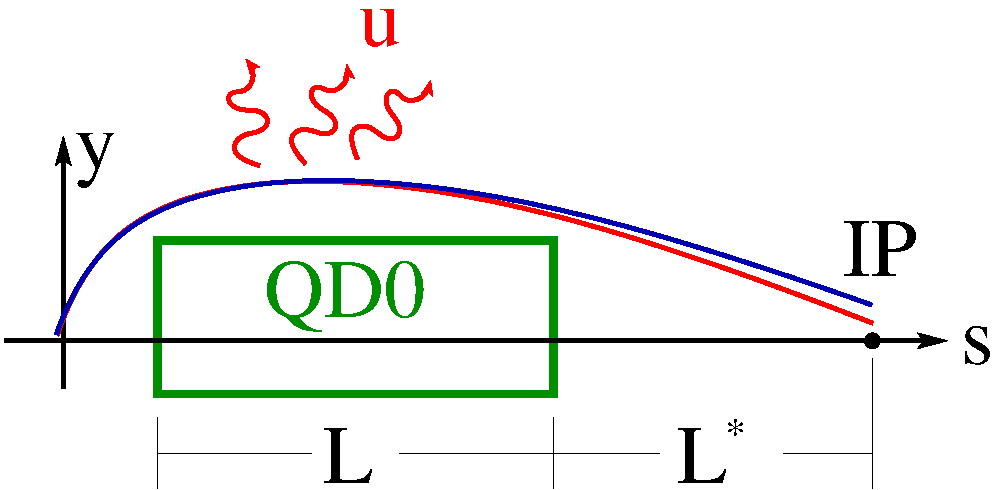
\includegraphics[scale=0.5]{Oide.pdf}
\centering
\caption{Design particle trajectory in blue and the trajectory of a particle due to radiation in the quadrupole in red.}\label{f:Oideeffect}
\end{figure}
 The beam size growth due to radiation is added quadratically to the linear beam size $\sigma_0^2=\epsilon\beta$ where $\beta$ represents the optical beta function and $\epsilon$ is the emittance. Therefore, $ \sigma^2 = \sigma_0^2 + \sigma_{oide}^2$, where the beam size contribution from the Oide effect is \cite{Oide},
 \begin{equation}
  \sigma^2_{oide} = \frac{110}{3\sqrt{6\pi}}r_e\frac{\lambda_e}{2\pi}\gamma^5 F(\sqrt{k}L,\sqrt{k}L^*)\left(\frac{\epsilon}{\beta^*}\right)^{5/2}
  \label{Oideequ}
 \end{equation}
 where
 \begin{equation}
  F(\sqrt{k}L, \sqrt{k}L^*) = \int_0^{\sqrt{k}L}|\sin\phi+\sqrt{k}L^*\cos\phi|^3\left[\int_0^\phi(\sin\phi'+\sqrt{k}L^*\cos\phi')^2 d\phi'\right]^2d\phi
  \label{OideF}
 \end{equation}
  and $\lambda_e$ is the Compton wavelength of the electron, $r_e$ is the classical electron radius, $\gamma$ is the relativistic factor, $\epsilon$ is the geometrical beam emittance, $\beta^*$ is the Twiss parameter at the observation point (in this case, the IP), and $k$, $L$ and $L^*$ are the quadrupole gradient, the quadrupole length and the distance to the observation point measured from the closest magnet face.\par
   Although the total contribution to beam size depends on the lattice and beam parameters, the minimum achievable beam size is given by \cite{Oide}
%the function $F$ is calculated only from quadrupole parameters. For this reason, $F$ will be used as figure of merit for a quadrupole.
\begin{equation}
 \sigma_{y \text{ min}} = \left(\frac{7}{5}\right)^\frac{1}{2}\left[\frac{275}{3\sqrt{6\pi}}r_e\frac{\lambda_e}{2\pi}F(\sqrt{K}L,\sqrt{K}L^*)\right]^\frac{1}{7}(\epsilon_{Ny})^\frac{5}{7}
\end{equation}
where $\epsilon_N=\gamma\epsilon$ is the normalized emittance, showing the independence from beam energy.\par
The only possibility to reduce the beam size is by changing the value of $F$, by modifying the magnet parameters, or to minimize the beam emittance. However, using the ILC 500 GeV \cite{ILCdes}, CLIC 500 GeV and CLIC 3 TeV \cite{CLICdes} parameters, it is possible to conclude from columns $\sigma_0$ and $\sigma_{oide}$ in Table (\ref{t:Sigmas}) that the contribution of the Oide effect to beam size is only significant for CLIC 3 TeV.\par
In addition, columns $\sigma$ and $\sigma_{min}$ in Table (\ref{t:Sigmas}) show that both CLIC designs are close to the minimum achievable beam size.\par
\begin{table}[!hbt]
\centering
{\scriptsize
\begin{tabular}{l||c|c|c||c|c|c|c|c||c|c}\hline\hline
Lattice &$\epsilon_N$& $\gamma$& $\sigma_0$&$k$&$L$&$L^*$& $F$ & $\sigma_{oide}$&$\sigma$&$\sigma_{min}$\\
 &(nm)&($10^3$)&(nm)&(m$^{-2}$)&(m)&(m)&&(nm) &(nm)&(nm)\\\hline
CLIC 3 TeV & 20 & 2935.0 & 0.70 & 0.116 & 2.73 &3.5&  4.086  & 0.85 & 1.10& 1.00 \\
CLIC 500 GeV & 25 & $\;\;$489.2 & 2.3 & 0.077 & 3.35 &4.3& 4.115 & 0.08 & 2.3 & 1.17\\
ILC  500 GeV & 40 & $\;\;$489.2 & 5.7 & 0.170 & 2.20 &4.3& 9.567 & 0.04 & 5.7 & 1.85\\\hline
\end{tabular}\caption{Vertical beam size and radiation beam size contribution for three lattices. $\epsilon_N$ is the normalized emittance, $\epsilon_N=\gamma\epsilon$.}\label{t:Sigmas}
}
\end{table}

\section{Oide Double Integral Solution}\label{s:DoubleIntegral}
In this section the double integral used to calculate $F$ is solved with the goal to increase the computational calculation speed. It was included in MapClass2\cite{Mapclassorig,Mapclass,Mapclass2,githubMapClass2} to be used in lattice design and optimization.\par
  The inner integral over $\phi'$ can be solved because it has a known primitive.
\begin{equation}
 \int_0^\phi (\sin \phi'+ \sqrt{k}l^*\cos\phi')^2d\phi'=\frac{\phi}{2}[(\sqrt{k}l^*)^2 +1 ] + \frac{\sin(2\phi)}{4}[(\sqrt{k}l^*)^2 -1]+\sqrt{k}l^*\sin^2\phi
\end{equation}
The Eq. (\ref{OideF}) can now be expressed as one integral.
{\scriptsize
\begin{align}
F(\sqrt{k}L&,\sqrt{k}l^*) =\\
&\int_0^{ \sqrt{k}L} |\sin\phi+\sqrt{k}l^*\cos\phi|^3 \left( \frac{\phi}{2}[(\sqrt{k}l^*)^2 +1 ] + \frac{\sin(2\phi)}{4}[(\sqrt{k}l^*)^2 -1]+\sqrt{k}l^*\sin^2\phi\right)^2 d\phi\notag
\end{align}
}
The squared factor in brackets is always positive because all inner terms are real. The term inside the absolute value is also always positive, therefore, the integrand is always positive. Now, considering the function:
  \begin{equation}
  |\sin \phi + \sqrt{k}l^*\cos\phi|=\left\{
  \begin{array}{c l l}
&  \sin\phi+\sqrt{k}l^*\cos	\phi,\quad\qquad&\text{if}, \sin\phi+	\sqrt{k}l^*\cos	\phi\geq0\\
&  -(\sin\phi+\sqrt{k}l^*\cos\phi),\quad&\text{if}, \sin\phi+	\sqrt{k}l^*\cos	\phi<0
  \end{array}\right.\label{eq-absval}
 \end{equation}
sign changes at every point $\quad\phi_n = \arctan(-\sqrt{ k}l^*)\pm n\pi,\quad n\geq1$.\par
It is possible to split the integration interval $i$ times, being $i$ the number of $\phi_n$ solutions where $0<\phi_n<\sqrt{k}L$. On each of those intervals, the absolute value definition can be removed and replaced by the corresponding expression in Eq. (\ref{eq-absval}), having only a difference in sign. By defining the primitive $\mathscr{F}$ in an interval where the factor inside the absolute value is positive it is possible to evaluate $F$ as it is shown in Eq. (\ref{eq-primeval}).
\begin{equation}
 F(\sqrt{k}L,\sqrt{k}l^*)= \mathscr{F}|_0^{\phi_1} - \mathscr{F}|_{\phi_1}^{\phi_2} +  \mathscr{F}|_{\phi_2}^{\phi_3} - \mathscr{F}|_{\phi_3}^{\phi_4}+ \cdots \pm  \mathscr{F}|_{\phi_i}^{\sqrt{k}L}\label{eq-primeval}
\end{equation}
The change of signs in each interval is only  given by the absolute value definition, then, it is simpler to add the absolute value of each contribution.
\begin{equation}
 F(\sqrt{k}L,\sqrt{k}l^*)= \bigr\vert\mathscr{F}|_0^{\phi_1}\bigr\vert + \bigr\vert\mathscr{F}|_{\phi_1}^{\phi_2}\bigr\vert +  \bigr\vert\mathscr{F}|_{\phi_2}^{\phi_3}\bigr\vert + \bigr\vert\mathscr{F}|_{\phi_3}^{\phi_4}\bigr\vert + \cdots +\bigr\vert\mathscr{F}|_{\phi_i}^{\sqrt{k}L}\bigr\vert
\end{equation}
If we know the primitive $\mathscr{F}$ and we are able to calculate the $\phi_n$s in the integration interval, then, it is possible to calculate the factor $F$ without using an approximate integrator. The double integration has been simplified to a primitive evaluation.\par
The primitive $\mathscr{F}$ exists and it has been calculated using Maxima \cite{Maxima} and Wolfram Alpha Mathematica\cite{Wolfram} software, the expression is in Appendix \ref{c:primitiveF}.\par
  
 
\section{Mitigating the impact on the beam size}
\subsection{QD0 length}
As shown in Sect. \ref{Oideeffect} the Oide beam size contribution depends on a combination of beam and optics parameters. %Table \ref{tabSigmas} gives the results.
If none of the beam parameters is to be changed then $F$ can be used as a figure of merit of the optics as it is calculated only from $k$, $L$ and $l^*$. The target is to reduce it as much as possible. Two energy cases are analyzed in the following: 3 TeV ($l^*=3.5$ m) and 500 GeV ($l^*=4.3$ m).\par
Columns $\sigma_0$, $\sigma_{oide}$ and $F$ in Table \ref{t:Sigmas} show that CLIC 3 TeV and 500 GeV \cite{CLICdes,TomasCLIC} have larger contributions to beam size even having a lower $F$ value than ILC 500 GeV \cite{ILCdes}.\par
In order to evaluate the minimum possible $F$ for $l^*$ given, the minimum $k$ required to get the particles focused is when the Twiss function $\alpha$ is zero just at the quadrupole opposite face to the IP.\par
Figure \ref{fig-3TeV:a}  shows the ratio squared between the beam size contribution due to Oide effect and the linear beam size for three cases: when $k$ is the minimum required to get particles focused (to get $\alpha_y=0$ at QD0 opposite side to the IP), when $k$ is calculated as thin lens ($k=\frac{1}{Ll^*}$), and the current QD0 status. Fig. \ref{fig-3TeV:b} shows the $k$ values for the previous mentioned cases.\par
The Oide contribution to beam size is of the same order of the linear beam size. It might be possible to reduce it by doubling the current quad length and using a lower $k$ between the minimum required for the focusing and the thin lens approximation. This also points to increasing the lattice length as this change reduces the tolerance to variations of $\alpha$ at the quadrupole input.\par
Quad lengths larger than 10 m do not lead to further improvements with the current parameters.\par

\begin{figure}[!htb]
\centering
\hspace*{-0.6cm}
\begin{subfigure}{0.45\textwidth}
\centering
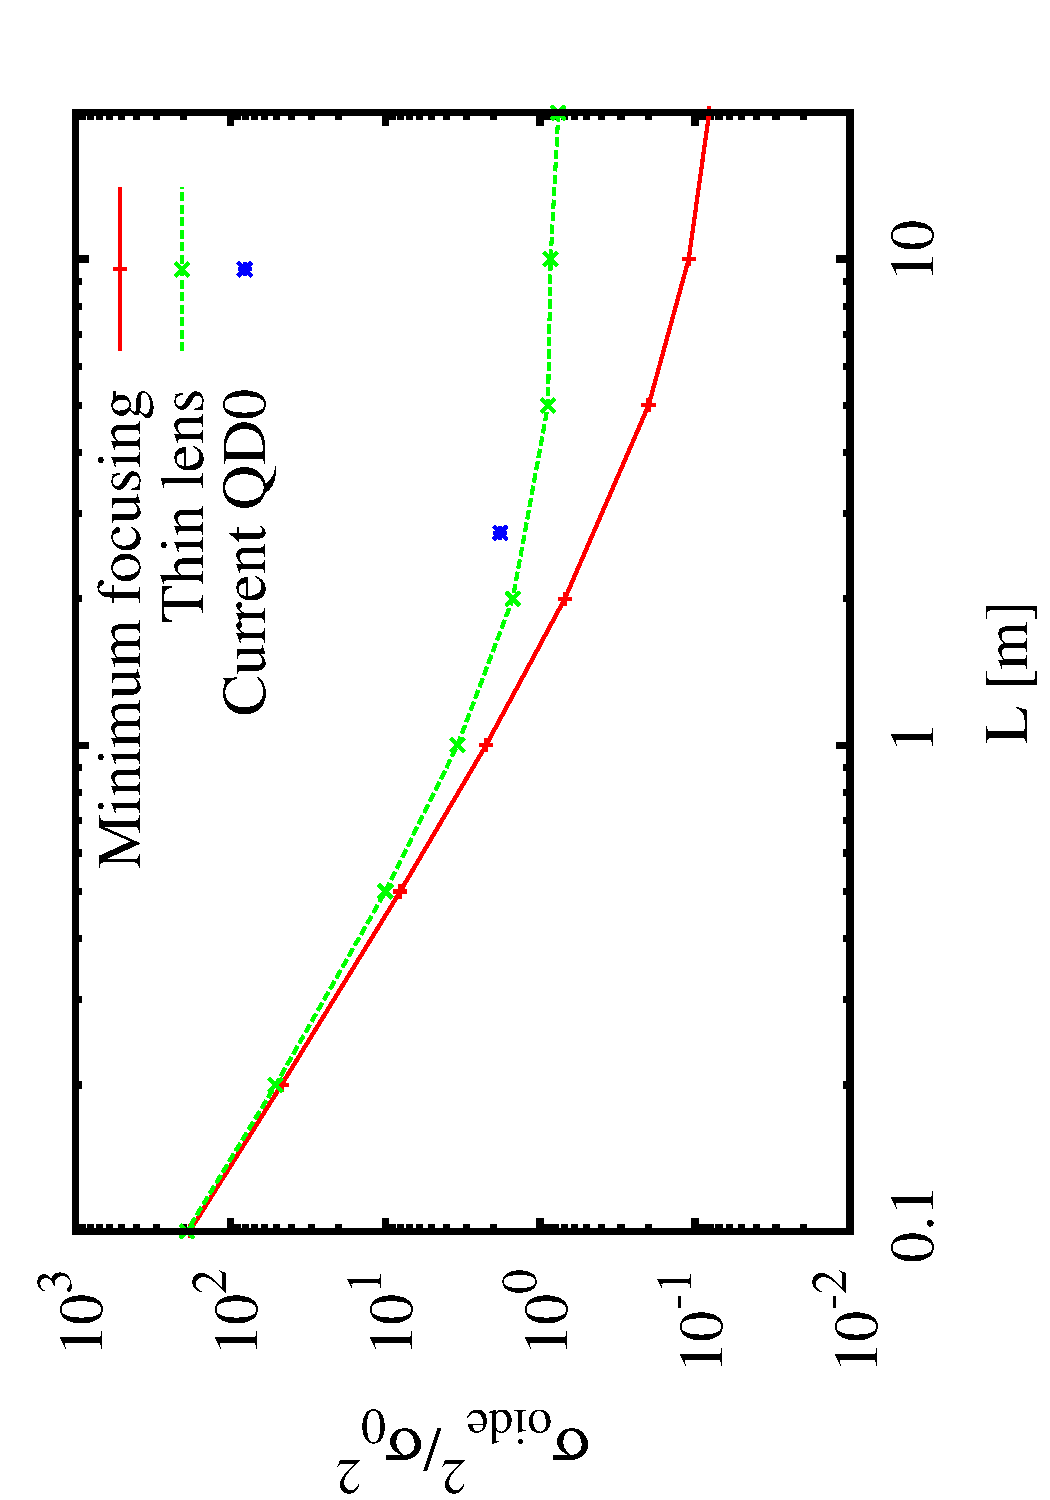
\includegraphics[scale=0.3,angle=-90]{image07a.pdf}\caption{}\label{fig-3TeV:a}
\end{subfigure}
\begin{subfigure}{0.45\textwidth}
\centering
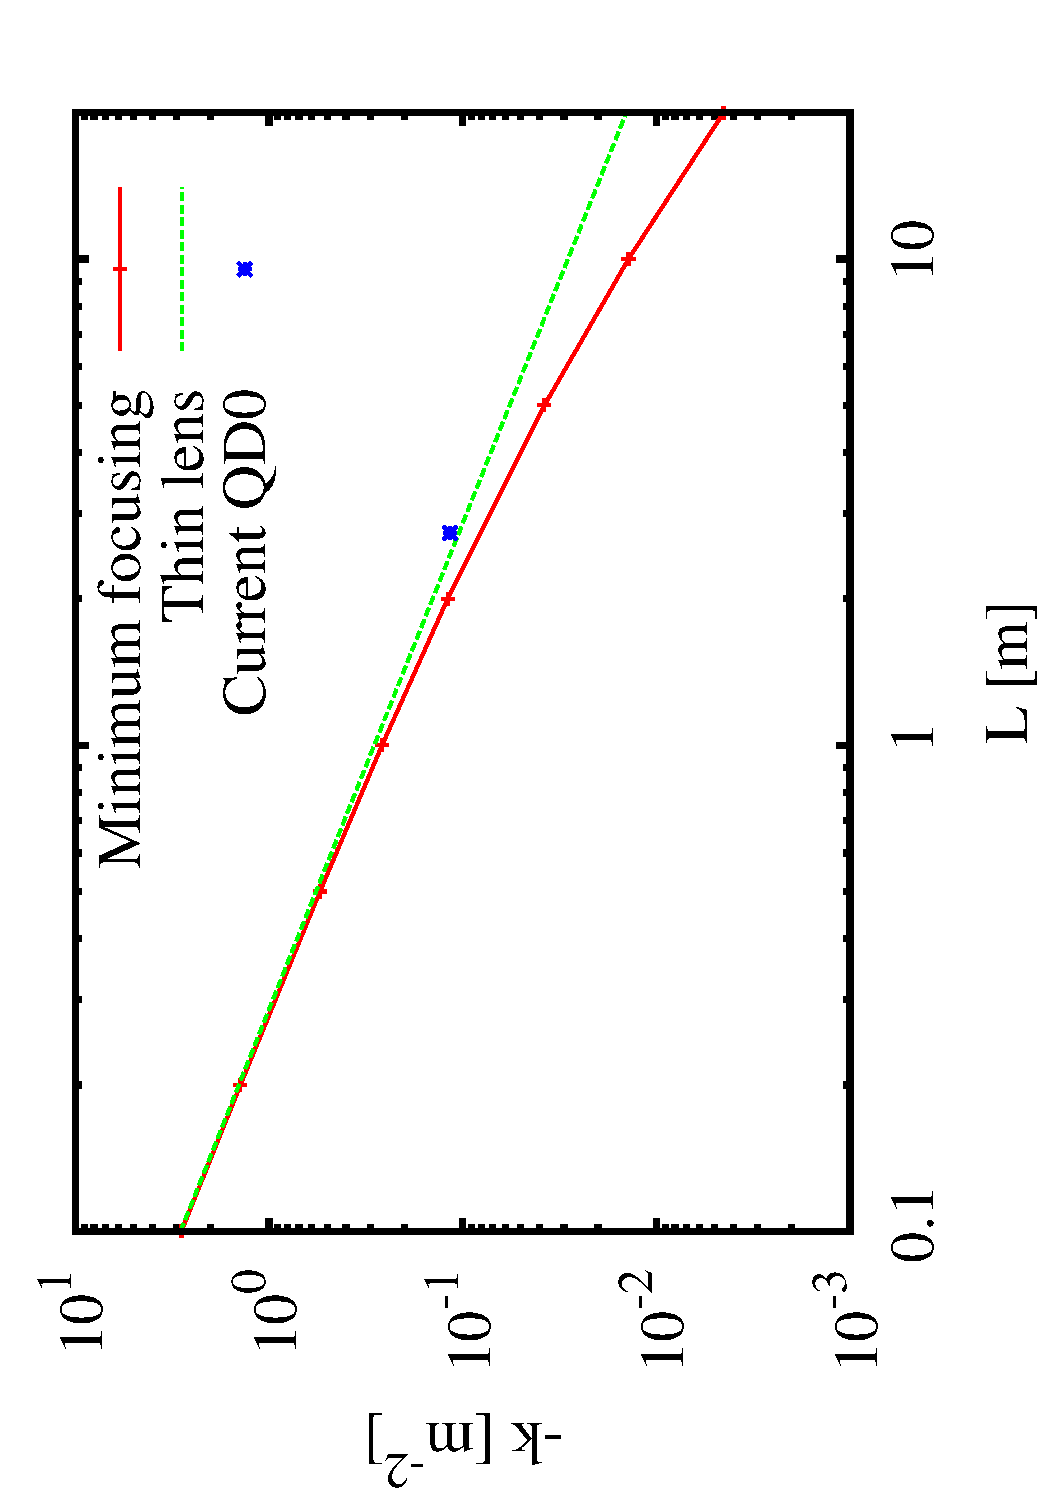
\includegraphics[scale=0.3,angle=-90]{image07b.pdf}\caption{}\label{fig-3TeV:b}
\end{subfigure}
\caption{Oide effect beam size contribution for CLIC 3 TeV design parameters. (a) $\sigma^2_{oide}$ normalized to designed linear beam size as a function of quad length for the minimum focusing $k$ (when $\alpha_y=0$ at the quadrupole opposite side to the IP), for $k$ calculated as thin lens ($k=\frac{1}{Ll^*}$) and the current QD0. (b) $k$ in the three previous cases for comparison.}\label{fig-3TeV}	
 \end{figure}\par
Figure \ref{fig-500GeV} is the corresponding to Fig. \ref{fig-3TeV} for the 500 GeV case. The current design contributes less than 4\% of the total beam size, concluding that the current QD0 length with the CLIC 500 GeV parameters does not need adjustment.\par
\begin{figure}[!htb]
\centering
\hspace*{-0.6cm}
\begin{subfigure}{0.45\textwidth}
\centering
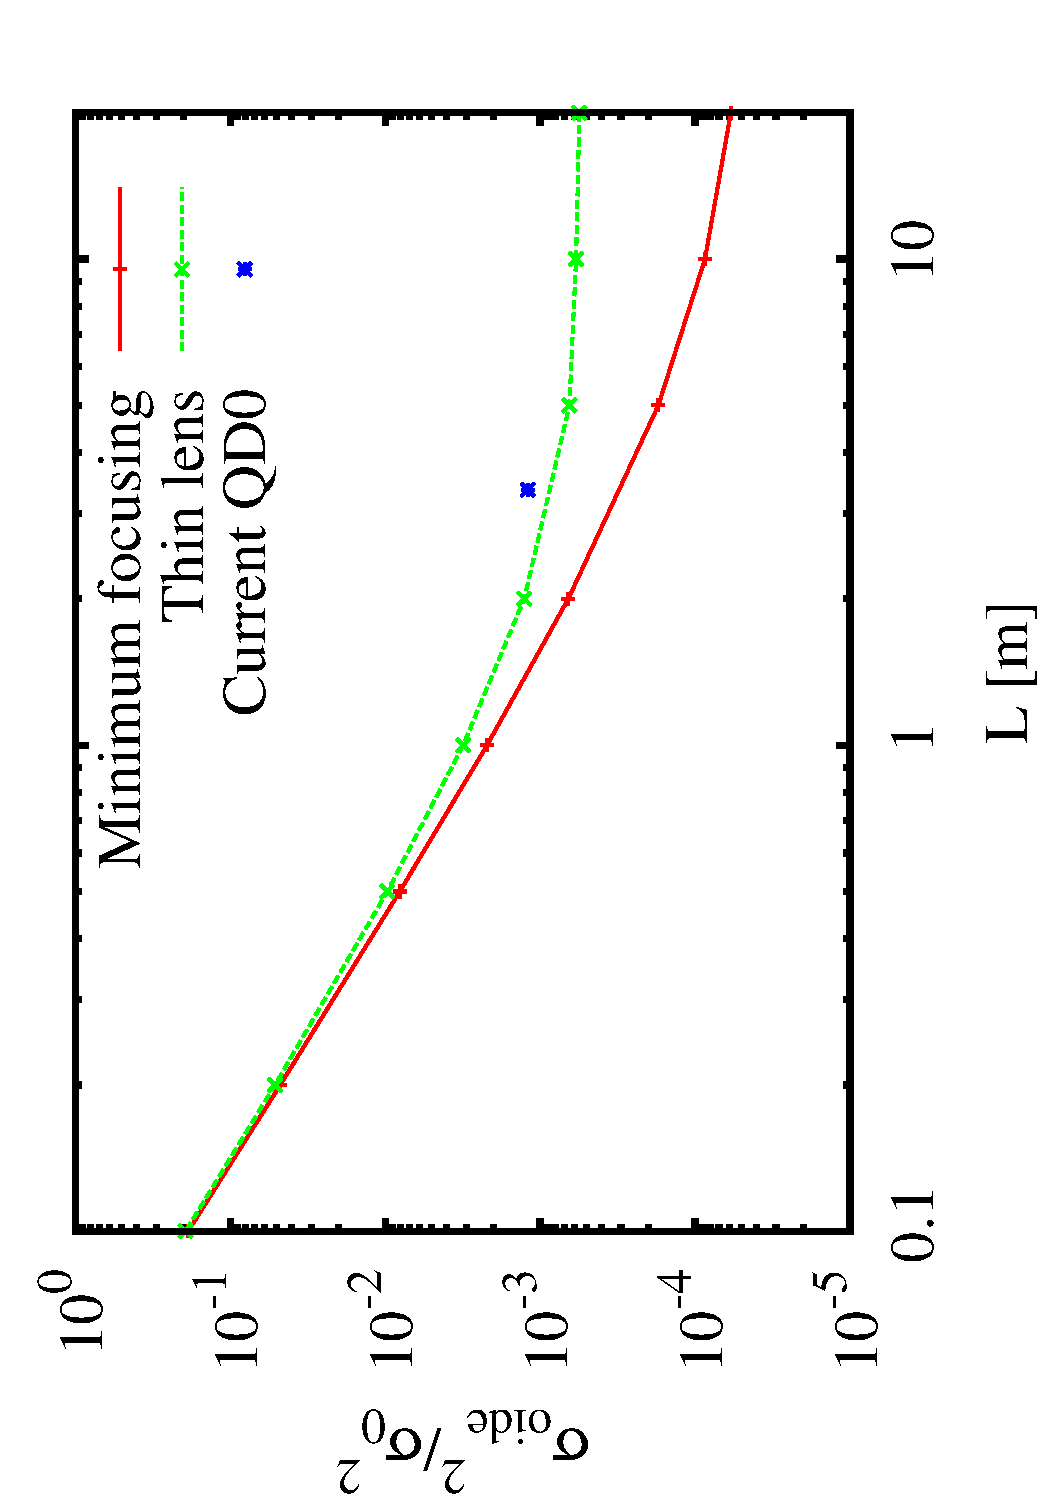
\includegraphics[scale=0.3,angle=-90]{image06b.pdf}\caption{}
\end{subfigure}
\begin{subfigure}{0.45\textwidth}
\centering
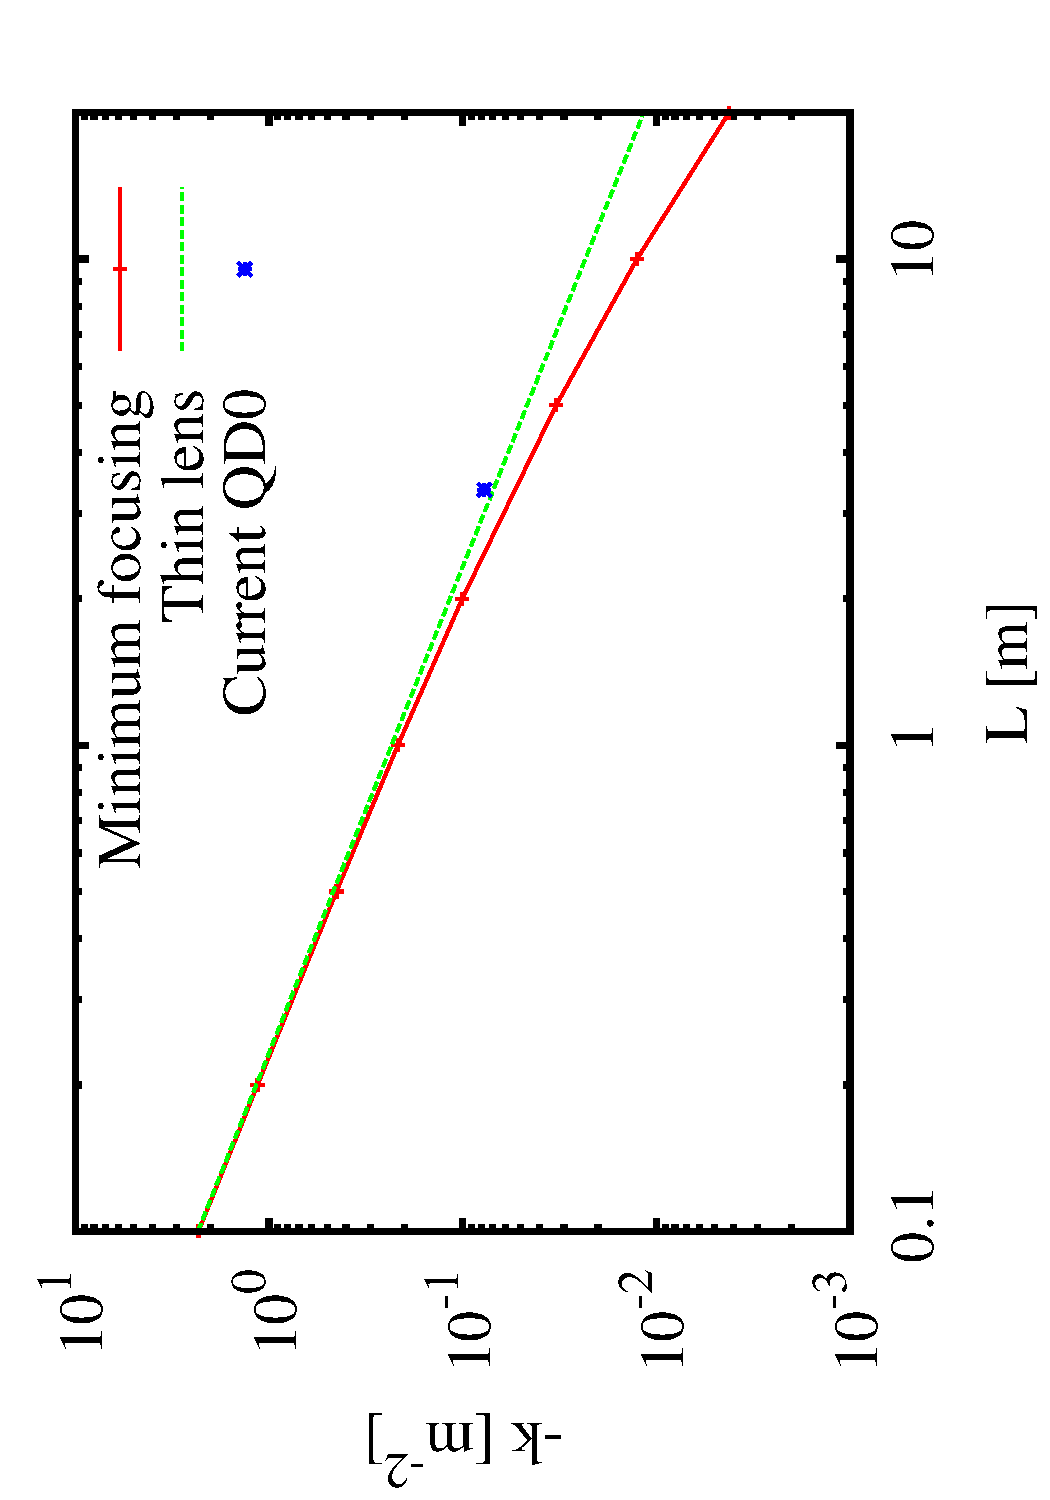
\includegraphics[scale=0.3,angle=-90]{image06c.pdf}\caption{}
\end{subfigure}
\caption{Oide effect beam size contribution for CLIC 500 GeV design parameters. (a) $\sigma^2_{oide}$ normalized to designed linear beam size as a function of quad length for the minimum focusing $k$ (when $\alpha_y=0$ at the quadrupole opposite side to the IP), for $k$ calculated as thin lens ($k=\frac{1}{Ll^*}$) and the current QD0. (b) $k$ in the three previous cases for comparison.}\label{fig-500GeV}
 \end{figure}\par	

\subsection{Correctors}
\subsubsection{$\Delta y$ due to radiation}
Particle tracking from the imput of QD0 to the IP for CLIC 3 TeV with and without radiation, using PLACET \cite{Placet}, allows one to compute the effects of radiation on the six dimentional phase space. Figure \ref{f:CLIC3TeVbeamsizeIP} shows the current transverse distribution of particles at the IP. To compensate the adverse effects a compensation system would ideally remove the position change due to radiation $\Delta y = y_\text{rad} -y_0$.\par
\begin{figure}[!htb]
\centering
 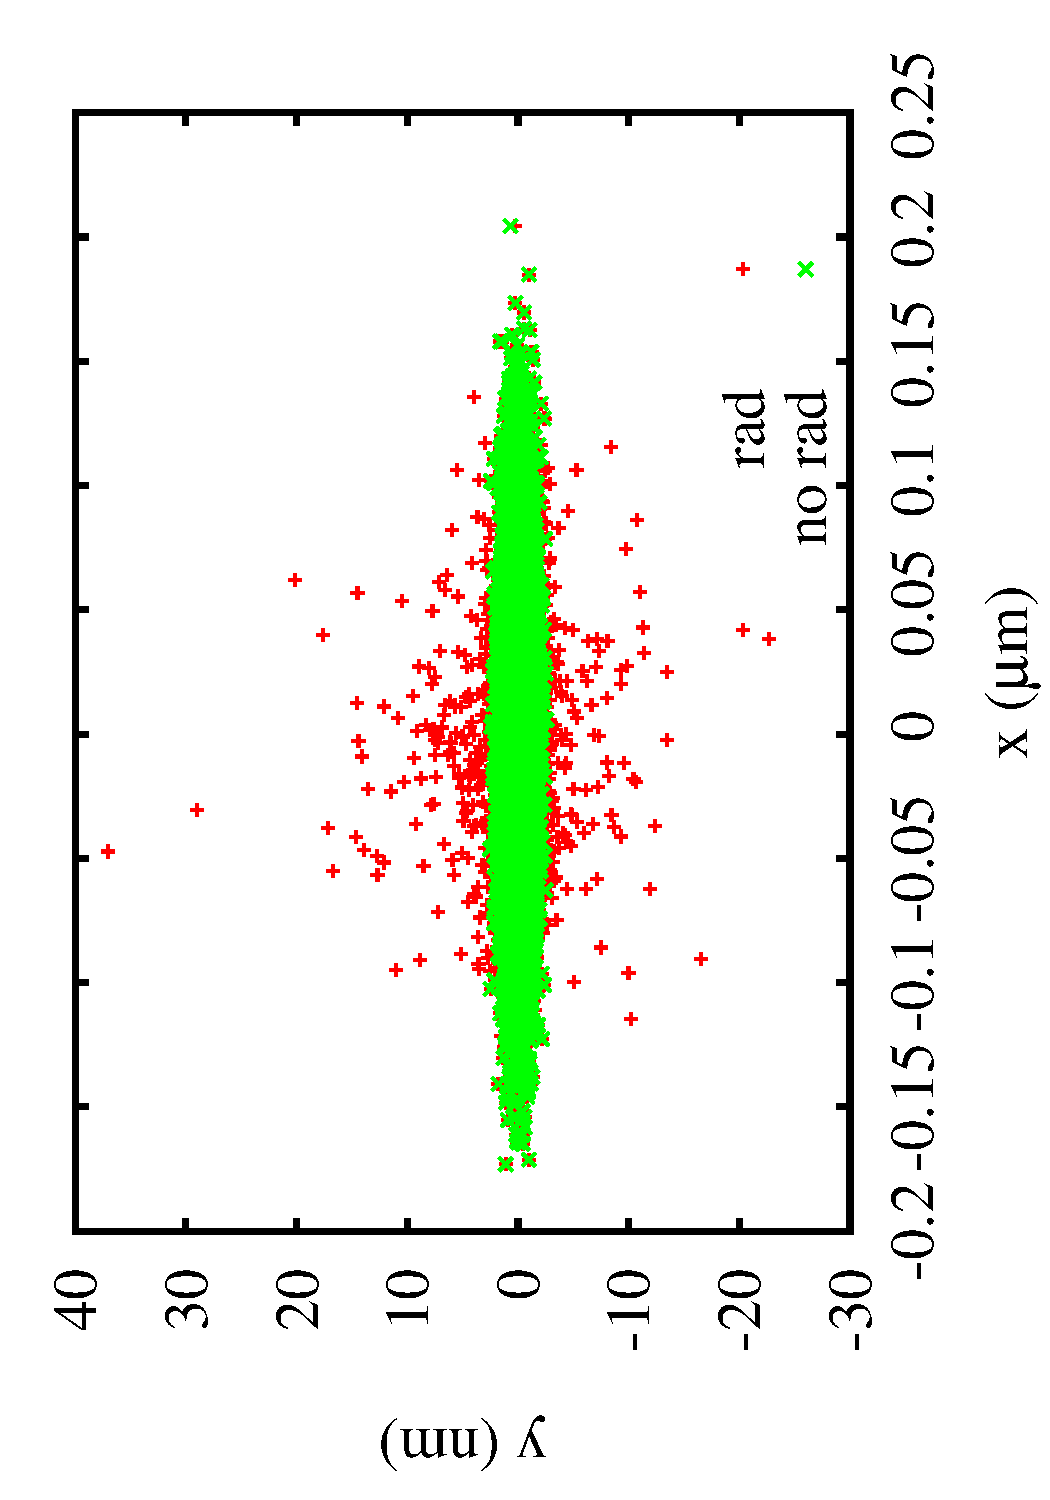
\includegraphics[scale=0.3,angle=-90]{plotxyrad.pdf}\caption{CLIC 3 TeV beam at the IP after tracking through 	QD0 with and without radiation.}\label{f:CLIC3TeVbeamsizeIP}
\end{figure}
Although the average radiation effect is zero, $\langle \Delta y \rangle = 0$ because of the cubic term $(y_0')^3$ as stated by Oide \cite{Oide}, the correlation between $\Delta y, y'$ is not zero. The correlation expression is shown in Eq. (\ref{eq:deltamean}).
\begin{equation}
 \langle\Delta y,y'_0\rangle = \frac{2}{3}r_e\gamma^3G(\sqrt{K}L,\sqrt{K}L^*)(y'_0)^3\label{eq:deltamean}
\end{equation}
%$r_e$ is the clasical electron radius and 
where $G(\sqrt{K}L,\sqrt{K}L^*)$ is given by
\begin{equation}
\int_0^{\sqrt{K}L}(\sin\phi+\sqrt{K}L^*\cos\phi)^2\int_0^\phi (\sin\phi'+\sqrt{K}L^*\cos\phi')^2 d\phi'd\phi
\end{equation}
Fig. \ref{f:correlation} shows the comparison between the correlation obtained from tracking and the theoretical evaluation of the previous expression.\par
\begin{figure}[!htb]
\centering
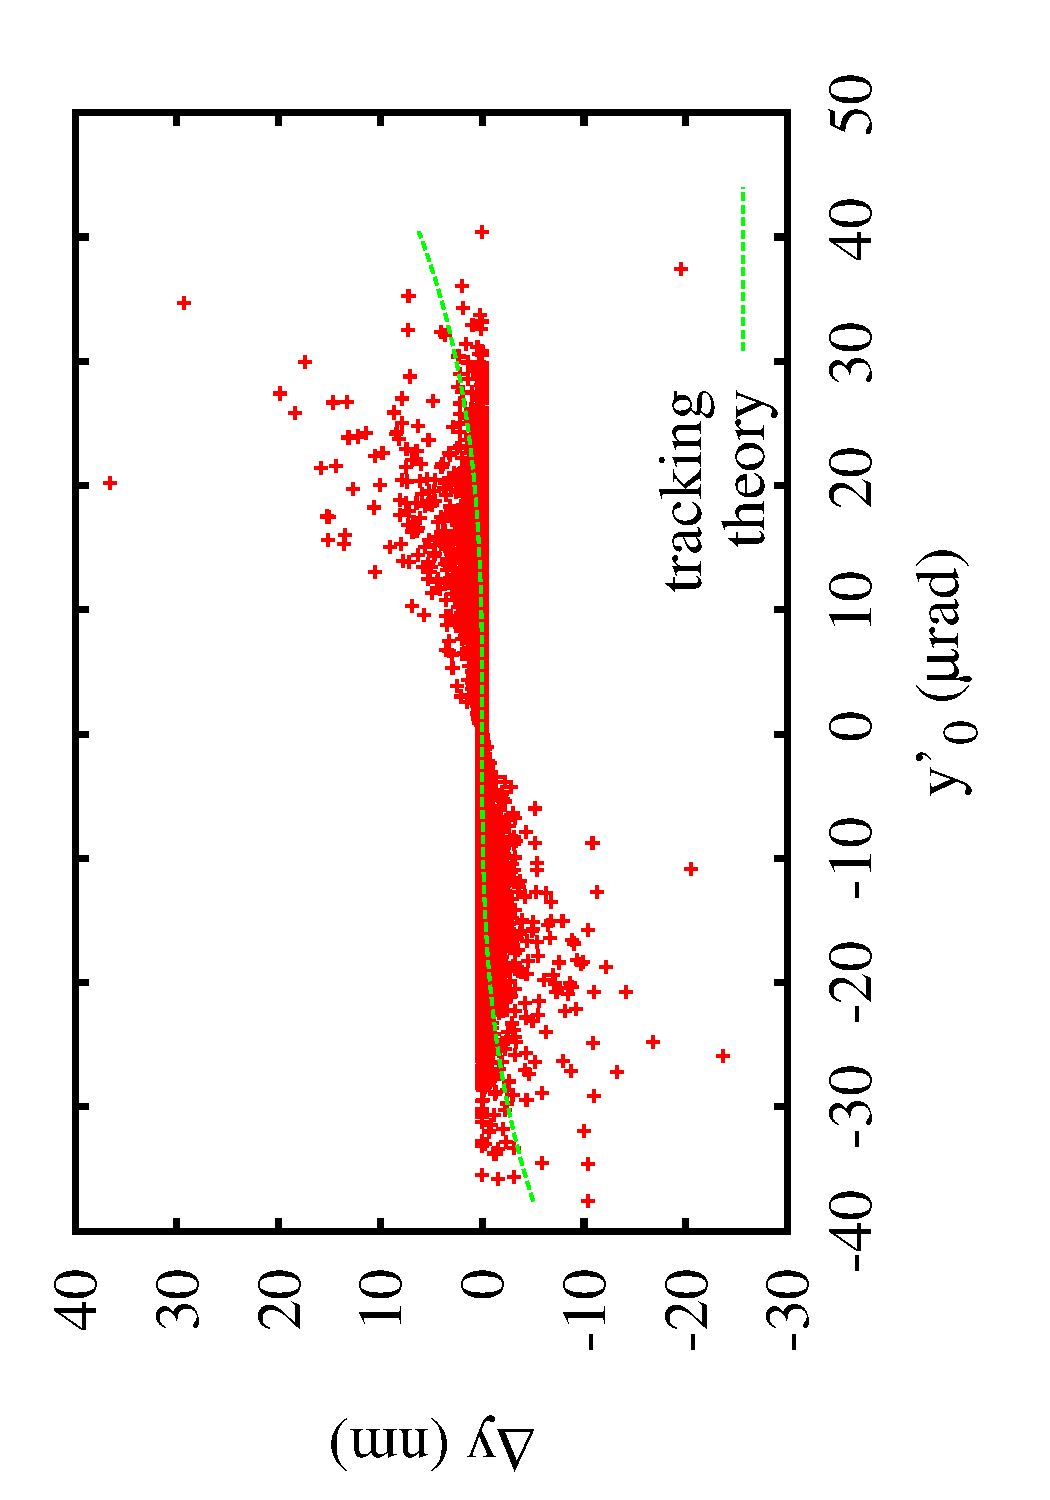
\includegraphics[scale=0.3,angle=-90]{plotdyrad.pdf}\caption{Correlation between the phase space coordinates $\Delta y,y'$ for CLIC 3 TeV from particle tracking and theoretical expression in Eq. (\ref{eq:deltamean}).}\label{f:correlation}
\end{figure}
This correlation could be removed from the beam size by a set of octupolar correctors to be presented in next Section.
\subsubsection{Correctors}
A pair of correctors, placed as in Fig. \ref{f:corrector}, is added to the strong focusing in order to mitigate the radiation effect. Particles that did not radiate along QD0 receive kicks in C1 and C0 cancelling one another. However, the C1 and C0 kicks do not cancel for particles that did radiate, this difference is used to correct only the particles trajectory change due to radiation.\par
The procedure consists in scaning the best position and multipole gradient ($s,k_i$) for C0, and then set C1 at QD0 input to cancel the effect of C0. If two points with same $\beta_y/\beta_x$ ratio are chosen, then the mutual cancellation of C1 and C0 correctors is limited only by the phase advance between them \cite{PhysRevSTAB.8.104002} and angle dispersion in the general case. Figure \ref{f:betaratio} shows the horizontal and vertical $\beta$ functions for CLIC 3 TeV in FD region, and their ratio.\par
The equal $\beta_y/\beta_x$ ratio for C0 and C1 condition is difficult to fulfill because C0 should be too close to the IP. In addition, it will lead to correctors running at very high strengths perturbing the beam.\par
A second approach is to minimize the phase advance between correctors. Therefore they will be located on both faces of QD0. This has the advantage of correctors running at lower strengths thanks to large $\beta$ functions.\par
\begin{figure}[!htb]
\centering
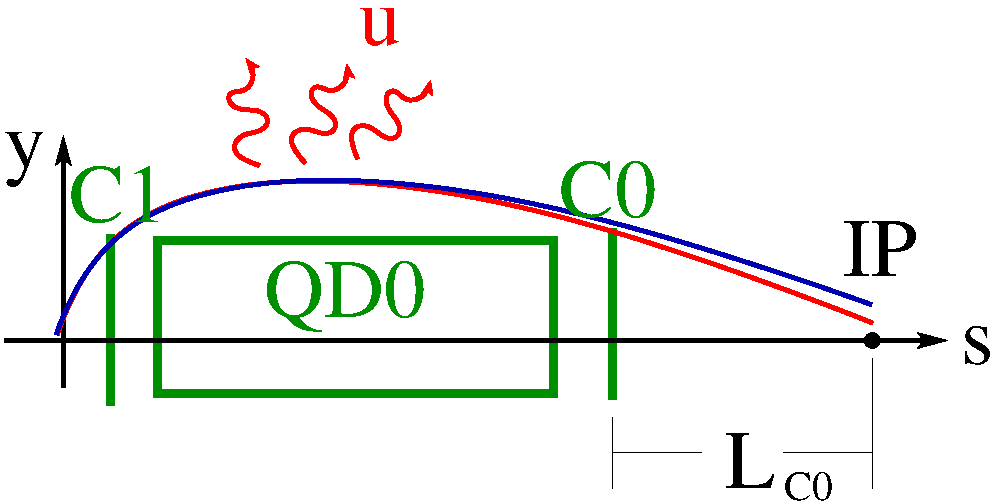
\includegraphics[scale=0.5,angle=0]{Oide2.pdf}\caption{For the nominal trajectory in blue, the kick in C1 must cancel the kick in C0. For all particles that radiate in red, the difference in kicks should cancel $\Delta y$.}\label{f:corrector}
\end{figure}
\begin{figure}[!htb]
\centering
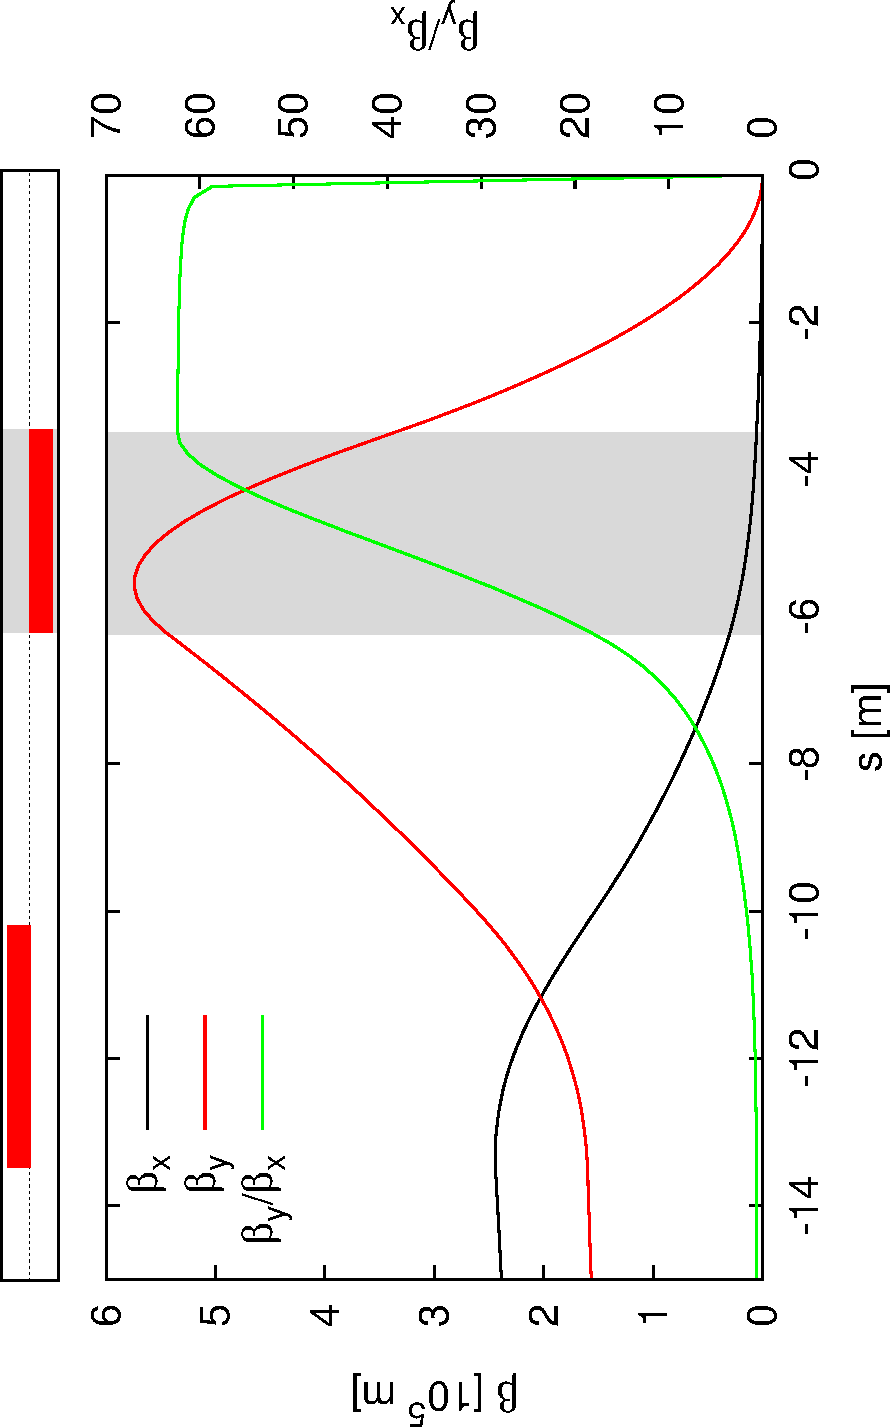
\includegraphics[scale=0.45,angle=-90]{lattice_CLIC_3TeVFD-crop.pdf}\caption{$\beta$ functions and $\beta_y/\beta_x$ ratio for CLIC 3 TeV FD, QF1 and QD0 in red on top. The dark area is occupied by QD0 and the IP is at $s=0$.}\label{f:betaratio}
\end{figure}
Two octupoles (OD0,OD1) were tried as correctors (C0,C1) to substract the cubic fit. A CLIC 3 TeV nominal beam with no energy spread is generated at the IP and tracked back to the entrance of the C1 without radiation with both correctors off. This beam is used to study the Oide effect mitigation in QD0 using correctors by tracking to the IP with radiation.\par
The best result obtained with the octupole correctors is a vertical beam size reduction by $(-4.3\pm0.2)$\% using OD0 only. Table \ref{t:correctors} shows the result of luminosity changes less than 10\% for the case with no radiation in QD0, with radiation, with one corrector and with the two correctors obtained with Guinea Pig ++ \cite{Schulte:382453}.\par
\begin{table}[!hbt]
\centering
\scriptsize
\begin{tabular}{c||c|c|c|c||c|c||c|c}\hline
& \multicolumn{2}{c|}{OD1} &\multicolumn{2}{c||}{OD0} & $\sigma_x$ & $\sigma_y$ & $L_{tot}$ & $L_{peak}$\\
& $L$ [m] & $k_3$ [m$^{-4}$] & $L$ [m] & $k_3$ [m$^{-4}$] &  [nm] & [nm] & \multicolumn{2}{c}{[$10^{34}$cm$^{-2}\cdot$ s$^{-1}$]}\\\hline\hline
NO RAD & 0.01 & 0 & 0.01 & 0 & 47.45 & 0.69 & 7.7 & 2.9\\
RAD    & 0.01 & 0 & 0.01 & 0 & 47.45 & 1.18 & 7.5 & 2.7 \\
RAD    & 0.01 & 0 & 0.01 & -3900 & 47.45 & 1.13 & 7.4 & 2.7 \\
RAD    & 0.01 & 1502 & 0.01 & -3900 & 47.45 & 1.17 & 7.1 & 2.7 \\\hline
% NO RAD & 0.01 & 0 & 0.01 & -3900 & 47.42 & 0.77 & - & -\\
% NO RAD & 0.01 & 1502 & 0.01 & -3900 & 47.42 & 0.75 & - & -\\\hline
\end{tabular}\caption{Effect of octupolar correctors on the beam size, total luminosity and peak luminosity.}\label{t:correctors}
\end{table}
The Oide effect contribution to vertical beam size affects very little the luminosity. The single corrector option., OD0, does not show any improvement in peak luminosities. However, the case of two correctors OD1 and OD0 shows a drop in the total luminosity. This has been attributed to the limited cancellation between correctors due to different $\beta_y/\beta_x$ ratio and phase advance.\par
The possibility of slicing QD0 in two or three sections and mitigate the radiation effect with a pair of octupoles on each/any slice could be studied.\par
\subsection{Conclusions}
Radiation in the final quad sets a limit on the vertical beamsize, this is called Oide effect. Only for CLIC 3 TeV this limit is significant, therefore two possibilities have been explored to mitigate its contribution to beam size: double the length and reduce the QD0 gradient, or the integration of a pair of octupoles before and after QD0.\par
The best result with octupoles demonstrated vertical beam size reduction of $(4.3\pm0.2)$\%, with little or negative impact on luminosity. The correction scheme is currently limited by the phase advance and $\beta_y/\beta_x$ ratio between correctors. It may be possible to improve its performance by slicing QD0.\par
